%!TEX root =../LibroTipoETSI.tex
\chapter{Introducción}\label{chp-01}


\lettrine[lraise=-0.1, lines=2, loversize=0.2]{E}{n} las prácticas de laboratorio realizadas
por parte de alumnos durante la docencia de los cursos de Robótica del Departamento de Ingeniería
de Sistemas y Automática de la Escuela Técnica Superior de Ingeniería de Sevilla, los alumnos
deben programar el movimiento de un brazo robótico presente en dicho laboratorio. El objetivo
es que una pieza sea trasladada por el robot desde un punto de la mesa de trabajo hacia una
segunda posición. El proceso se realiza colocando manualmente la pieza, con los problemas que
ello conlleva. Por un lado, la precisión es cuestionable, ya que el propio alumno no tiene una
referencia sobre la cual poder repetir el proceso de forma eficaz y el error introducido al sistema
es alto. Por otro lado, al invadir el espacio de trabajo del brazo robótico continuamente se
producen riesgos innecesarios impropios de las normas de seguridad en la industria.

Este trabajo es la continuación de \cite{tapia} y \cite{rea}, que sentaron las bases del proyecto.
En esta ocasión, el enfoque es en la implementación sobre los equipos del laboratorio. Por ello,
el sistema creado debe quedar en una caja donde se realicen las conexiones electrónicas y todos
los dispositivos. Además el sistema debe tener componentes fácilmente sustituibles para facilitar
las reparaciones.

El sistema cuenta con las siguientes características:
\begin{itemize}
	\item Posicionamiento de piezas en medidas de ejes X e Y que el usuario requiera para 
	interactuar con el robot.
	\item Conexión entre Arduino y RobotStudio mediante protocolo TCP/IP para comunicaciones.
	\item Funcionamiento sin Arduino mediante señales digitales del robot.
	\item Funcionamiento sin conexión directa entre RobotStudio y Arduino.
\end{itemize}

\section{Modos de funcionamiento}\label{sec-00}

Todas las funciones especificadas no pueden cumplirse al mismo tiempo ya que existirían conflictos
entre las mismas, por lo que el sistema debe tener ciertos modos de funcionamiento en los que
se activen o desactiven dichas características. 

La primera consideración es determinar el dispositivo que gobierna el sistema o \textit{máster}.
Por ello, se puede diferenciar cuando el máster es la controladora del robot (o RobotStudio durante
una simulación) o el sistema caja (Arduino o la propia electrónica interna). Respectivamente serán
los modos remoto y local.

Por otro lado, como el microcontrolador presente en el Arduino puede estar funcionando o no, se
deben añadir las dos posibilidades. Se tiene el modo con microcontrolador y sin microcontrolador.

En total, se cuenta con cuatro modos de funcionamiento que se describen a continuación.

\subsection{Modo local con microcontrolador}\label{subsec-01}

Las órdenes del sistema están proporcionadas por los periféricos de entrada presentes en la caja y
el microcontrolador es el encargado de gestionar el posicionamiento y mover el motor cuando
le sea indicado.

En caso de que esté disponible la conexión con la controladora del robot, el Arduino comunica 
mediante conexión TCP/IP la posición de la pieza en los ejes X e Y además del estado
del sensor fotoeléctrico y del sistema.

\subsection{Modo remoto con microcontrolador}\label{subsec-02}

El gobierno del sistema pasa a ser parte de la controladora del robot, convirtiendo al microcontrolador
en esclavo. El microcontrolador sigue encargándose del posicionamiento y movimiento del motor, pero las
órdenes pasan a ser recibidas mediante conexión TCP/IP.

Como en el caso anterior, se envía la posición, estado del sistema y del sensor fotoeléctrico mediante
conexión TCP/IP a la controladora.

\subsection{Modo local sin microcontrolador}\label{subsec-03}

Al no tener el microcontrolador operativo, el posicionamiento deja de funcionar y las funciones del
sistema pasan a ser más básicas. El movimiento del motor queda a cargo de la electrónica interna del
sistema. Para interactuar con el motor y moverlo se realizará mediante los pulsadores de avance y 
retroceso.

El robot queda no comunicado y solo recibe la señal digital del sensor fotoeléctrico.

\subsection{Modo remoto sin microcontrolador}\label{subsec-04}

Es un modo similar al anterior, en la cual la interacción con el sistema se produce mediante señales
digitales enviadas por el robot.

\begin{figure}[htbp]
	\centering
	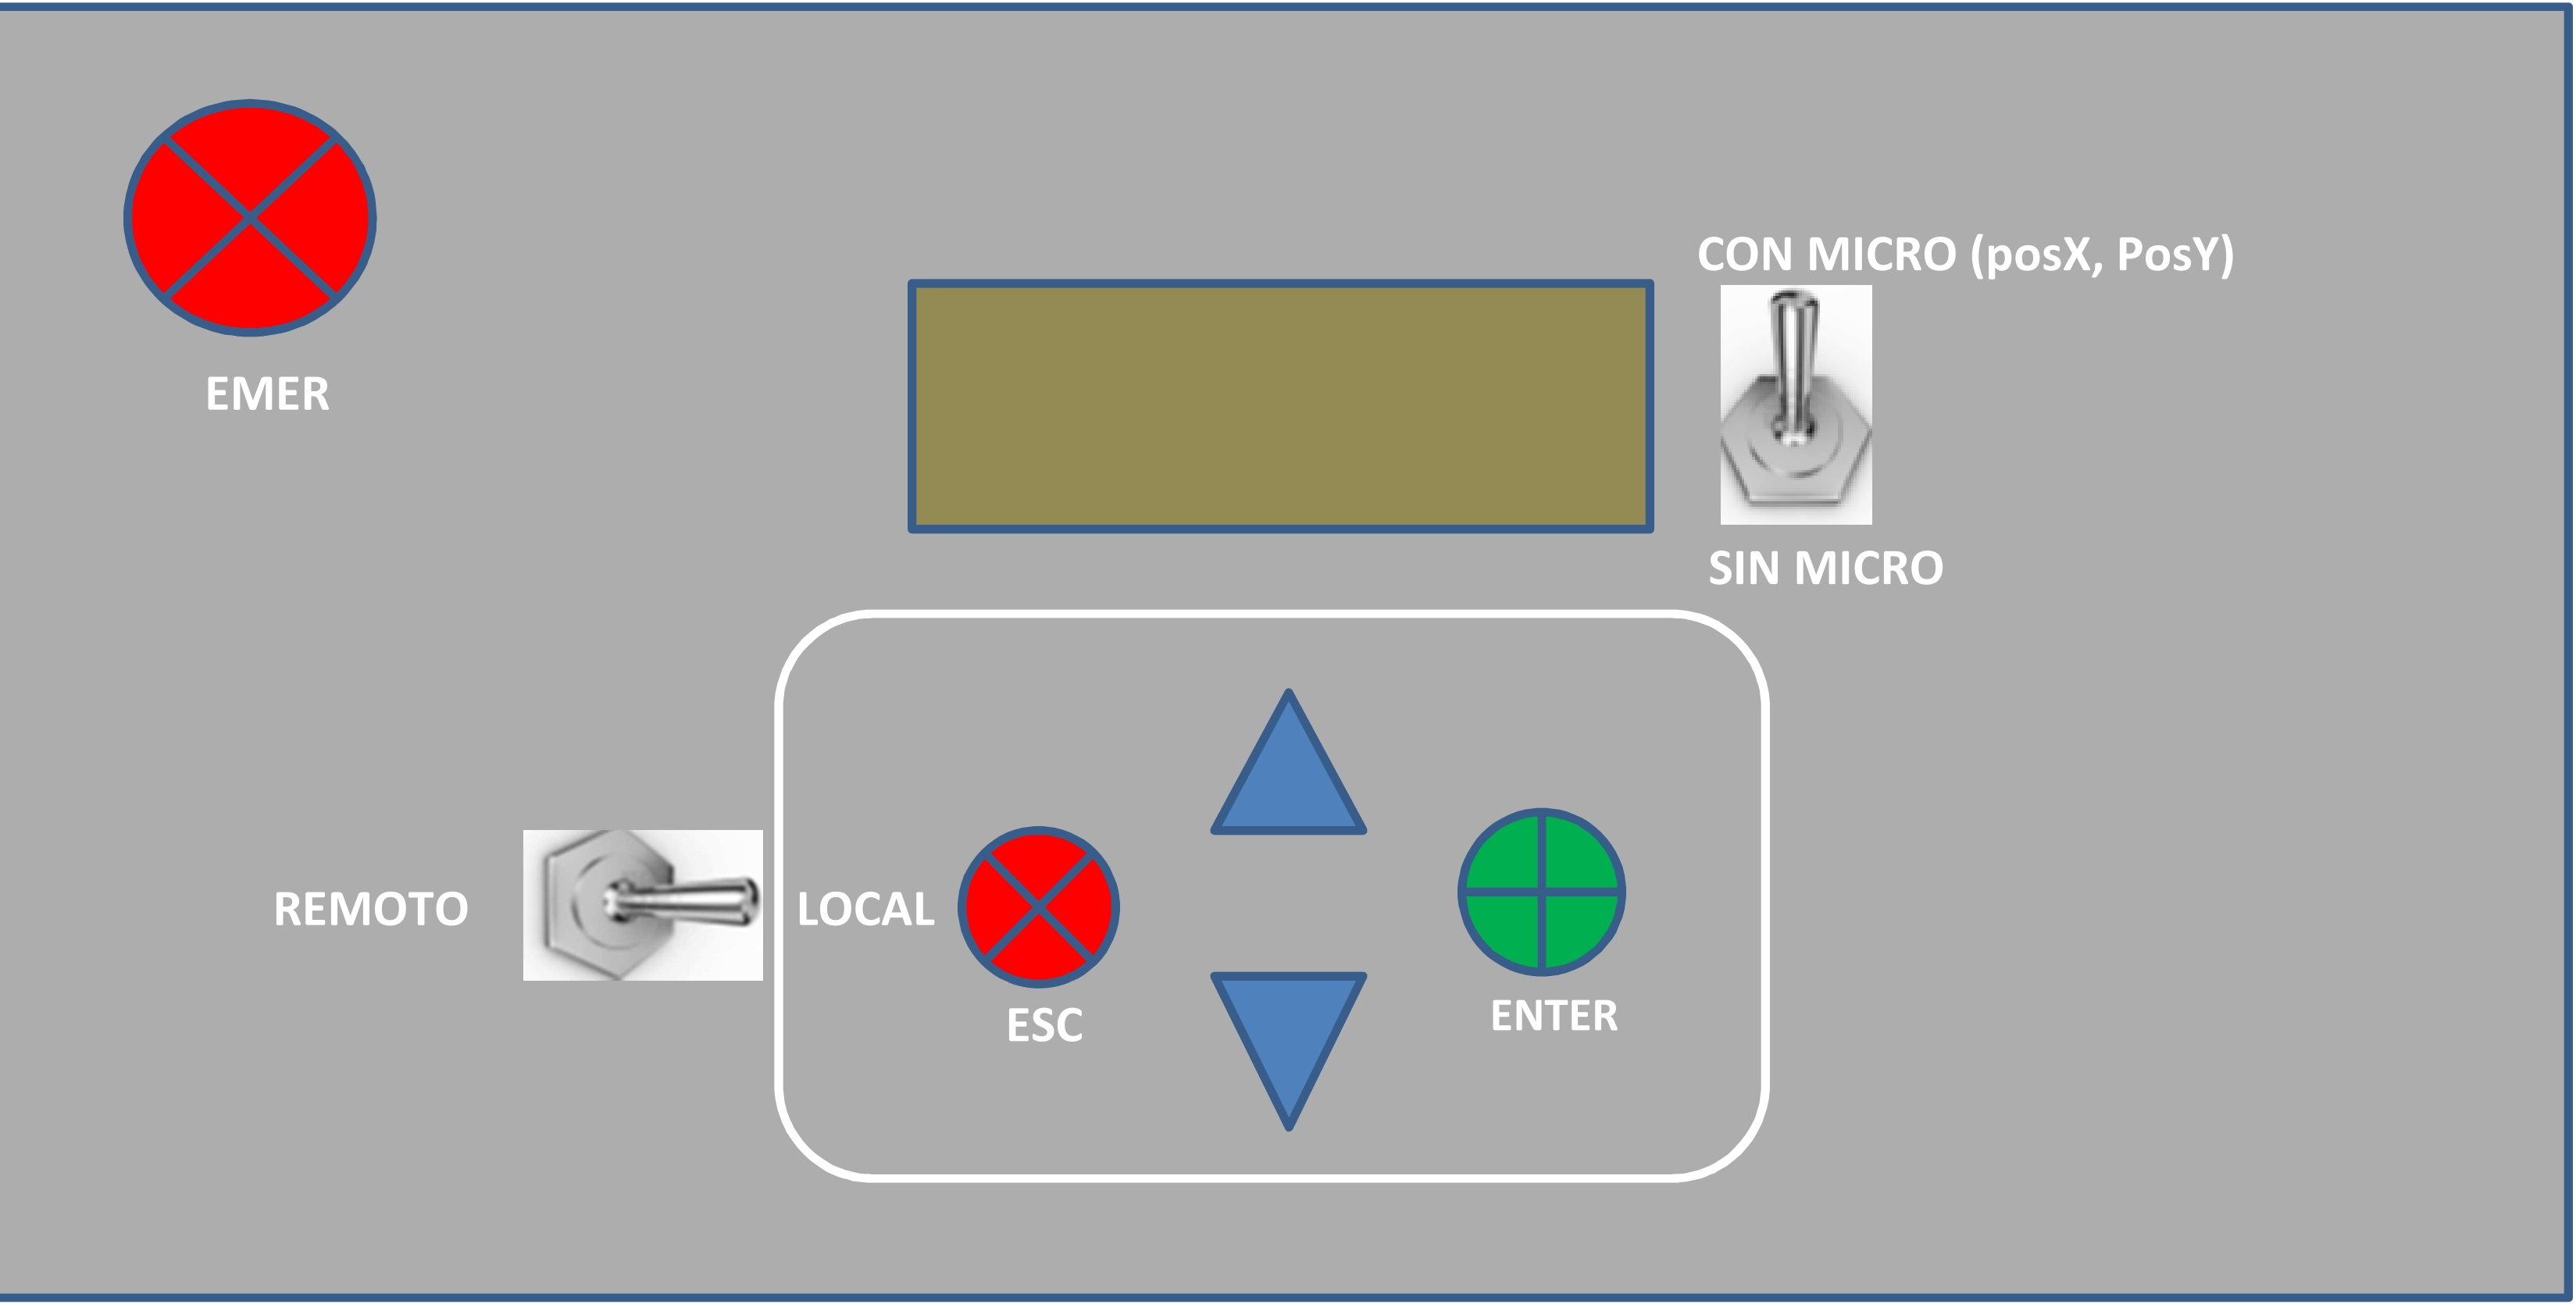
\includegraphics[width=\linewidth]{01-introduccion/botonera.jpg}
	\caption{Estructura de un aplicación que use la plataforma}
	\label{fig:figura1}
	\end{figure}
	

